\section{Bilag}

\begin{figure}[H] 
	\center
	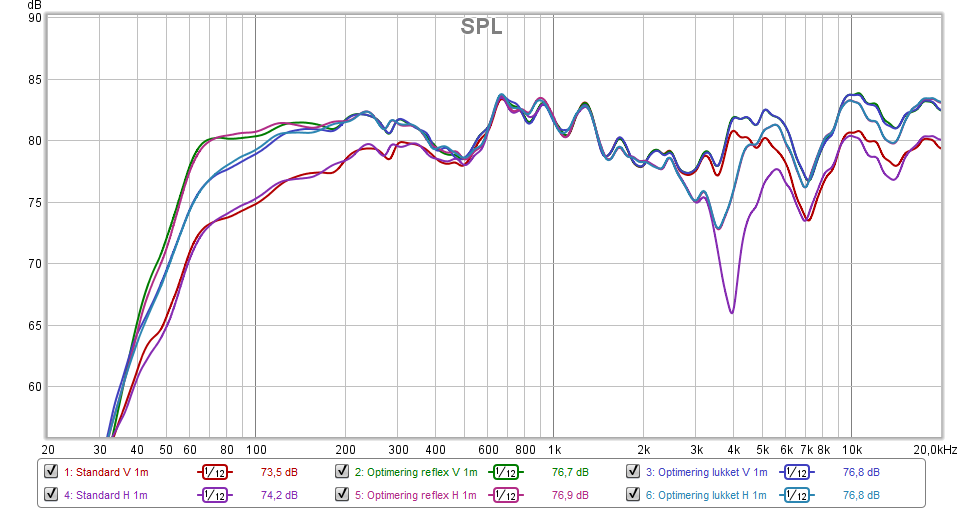
\includegraphics[width=1\linewidth]{figur/Optimering-forskel-VH}\quad
	\caption{Frekvenskarakteristik af både venstre og højre side med optimering/korrektion, Rød = venstre udgangspunkt med åben basrefleks, Grøn = venstre side optimeret med åben basrefleks, Blå = venstre side optimeret med lukket basrefleks, Lilla = højre side udgangspunkt med åben basrefleks, Pink = højre side optimeret med åben basrefleks, Cyan = højre side optimeret med lukket basrefleks}
	\label{fig:Optimering-forskel-VH}
\end{figure}

\begin{figure}[H] 
	\center
	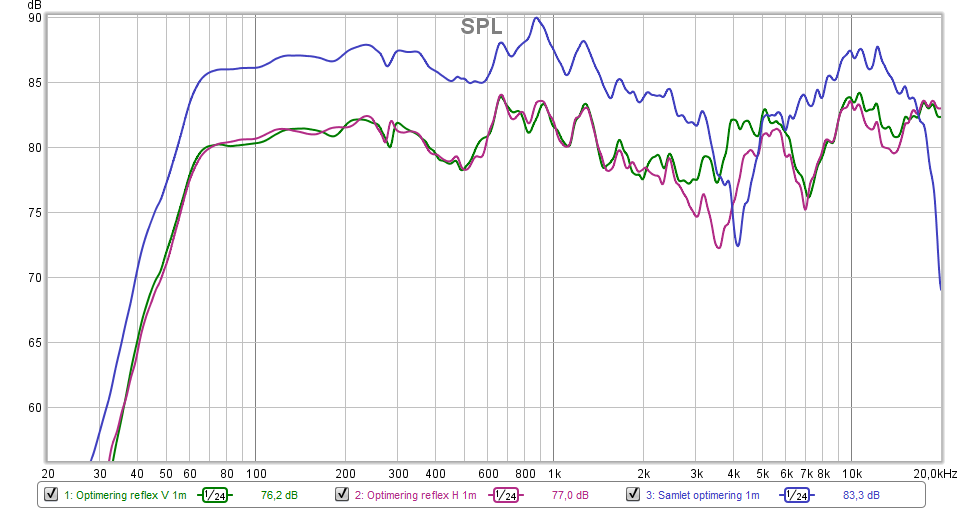
\includegraphics[width=1\linewidth]{figur/Samlet-Optimering}\quad
	\caption{Frekvenskarakteristik af venstre og højre side med optimering/korrektion samt den samlede højtaler. Grøn =  venstre side optimeret med åben basrefleks, Pink = højre side optimeret med åben basrefleks, Blå = den samlede højtaler optimeret med åben basrefleks}
	\label{fig:Samlet-Optimering}
\end{figure}

\newpage
\begin{lstlisting}[frame=single, caption={FIR EQ Matlab code},label={lst:matlab},captionpos=b]
%% AUTE FIR filter for EQ of project
Fs=44100;
taps = 1024;

% EQ Frequency axix
f = [0 20 25 31 40 50 60 80 100 125 160 200 250 315 400 500 630 800 1000 1250 1600 2000 2500 3150 4000 5000 6300 8000 10000 12500 16000 20000 Fs];
f_matlab = [0 20 25 31 40 50 60 80 100 125 160 200 250 315 400 500 630 800 1000 1250 1600 2000 2500 3150 4000 5000 6300 8000 10000 12500 16000 20000 Fs/2];

%normaliseret frekvens
fn = f/Fs;
fn_matlab = f_matlab/(Fs/2);
db6=6;
db3=3;
cut3 = 10^(-db3/20);
boost3 = 10^(db3/20);
cut6 = 10^(-db6/20);
boost6 = 10^(db6/20);

%% Jazz
EQ = ones(1,length(fn));
EQ(6:9)=cut3; %50-100 
EQ(11:15)=boost6; %160-400
EQ(17:18)=boost6; %630-800
EQ(22:26)=boost3; % 2000-5000
EQ(28:29)=boost3; % 8000-10000

b = fir2(taps, fn,EQ);
h = b;

b_matlab = fir2(taps, fn_matlab, EQ);
[H, f_vector] = freqz(b_matlab,1,20000, Fs);

figure
Hdb = 20*log10(abs(H));
semilogx(f_vector, Hdb);
grid on
axis([20 20000 -9 9])
title('Amplitudespektrum FIR filter Jazz');
xlabel('Frequency (Hz)');
ylabel('Magnitude (dB)');

for c = 1:length(h)
Jazz_tekstfil(c) = h(c)+",";
end

Jazz_tekstfil = Jazz_tekstfil';

%% Rock
EQ = ones(1,length(fn));
EQ(7:9)=boost6; %60-100 
EQ(12:13)=boost6; %200-250 
EQ(14:15)=cut6; %315-400 
EQ(16:22)=boost3; %500-2000
EQ(25:26)=boost6; %4000-5000
EQ(28:29)=boost6; % 8000-10000
EQ(29:end)=boost3; % 10000-end

b = fir2(taps, fn,EQ);
h = b;

b_matlab = fir2(taps, fn_matlab, EQ);
[H, f_vector] = freqz(b_matlab,1,20000, Fs);

figure
Hdb = 20*log10(abs(H));
semilogx(f_vector, Hdb);
grid on
axis([20 20000 -9 9])
title('Amplitudespektrum Fir Filter Rock');
xlabel('Frequency (Hz)');
ylabel('Magnitude (dB)');

for c = 1:length(h)
Rock_tekstfil(c) = h(c)+",";
end

Rock_tekstfil = Rock_tekstfil';
\end{lstlisting}



\begin{figure}[H] 
	\center
	\includegraphics[width=0.9\linewidth]{figur/Lyttetest}\quad
	\caption{Lyttetest formular}
	\label{fig:Lyttetest}
\end{figure}